% !TEX root = ../main.tex

\chapter{Introduction}
\label{ch:introduction}
Machine learning, particularly deep learning using neural networks, has greatly benefitted from the availability of large amounts of data. Neural networks have demonstrated significant potential in solving a wide range of tasks. By examining the potential of binary trees, this thesis aims to provide insights into alternative models that could complement or even surpass the performance of traditional neural networks in certain reinforcement learning scenarios.

\section{Neural Networks}

Neural networks are a type of machine learning that takes inspiration from the structure and function of neurons in the human brain. The model is composed of layers of interconnected artificial neurons, which process and transmit information. In neural networks, the input data is first passed through the first layer, and then each subsequent layer receives the output from the previous layer as input.

Neural networks learn by adjusting the connections, or weights, between neurons based on the input data and the desired output. The output of a single neuron is calculated by combining the inputs from the previous layer with the corresponding weights, and adding a bias term if applicable. This weighted sum is then passed through an activation function, which transforms the sum into the output of the neuron. Common activation functions include the sigmoid function, hyperbolic tangent (tanh), and rectified linear unit (ReLU). The choice of activation function depends on the specific task and the architecture of the network.

A neural network can be represented as a computational graph that combines a series of simple functions to produce complex and high-dimensional representations, which capture the underlying function that enables the network to make accurate predictions. This ability to learn multiple levels of abstraction through function composition is one of the key strengths of neural networks and sets them apart from traditional linear models. Figure \ref{fig:neural_network} illustrate a human-readable way to represent neural networks.

\begin{figure}[!ht]
\centering
\fbox{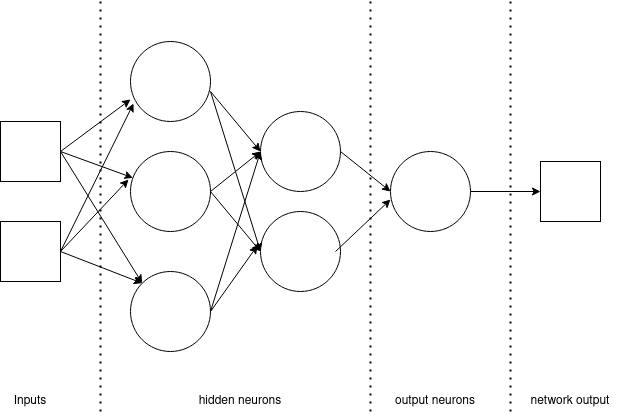
\includegraphics[width=.8\textwidth]{neural_network}}
\caption[Neural network representation]{
  \textbf{Neural network illustration}which process incoming input data through a structure consisting of two hidden layers, one with three neurons and one with two, and an output layer with a single neuron. The output produced by the network is determined by passing it through an activation function, which represents the final output of the network.
  }
\label{fig:neural_network}
\end{figure}


The most widely used optimization algorithm for the learning process is gradient descent, which helps find the optimal weights by minimizing the error between the network's predictions and the actual output. Backpropagation is a powerful tool for efficiently calculating the gradient of the loss function with respect to the weights. This is done through a forward pass, where the predicted outputs and intermediate node values are determined, followed by a backward pass, where the gradient of the loss function with respect to each weight is calculated using the chain rule of calculus. The gradient is then used to update the weights through gradient descent until the weights converge to values that minimize the loss function. For backpropagation to be effective, the activation functions of the artificial neurons must be continuous and easily differentiable (\cite{goodfellow_deep_2016}).

The structure of a neural network, including the number of layers and number of neurons per layer, significantly impacts its ability to solve tasks. A larger number of layers allows for the approximation of more complex functions, but can also result in overfitting, where the model performs well on training data but poorly on new data. The field dedicated to finding optimal structures is referred to as neural architecture search.

\section{Binary trees}

Trees are a type of data structure that are commonly used in computer science and mathematics. They consist of nodes, which are connected by edges. Trees can be seen as a special type of graphs that are undirected, connected, and acyclic, meaning that nodes are connected by edges, but there are no loops or cycles in the graph.

In a tree, each node is either a parent or a child. The top node, with no parent, is called the root, while the bottom nodes with no children are called leaves. The distance from the root node determines the level of the node, with the root at level 0 and its children at level 1, and so on. Nodes on the same level are called siblings.

Binary trees are a specific type of tree in which every node, except for leaves, has at most two children, which are called the left and right nodes. Binary trees are easy to understand and visualize, making them useful for a variety of applications. An example of a binary tree is shown in Figure \ref{fig:binary_tree}.

In addition to binary trees, there are other types of trees that are commonly used in computer science and data structures. One example is the "n-ary" tree, which allows nodes to have any number of children. Another example is the "balanced" tree, which is designed to keep the tree's height as small as possible, while still allowing for efficient searches and insertions. Balanced trees come in several different varieties, such as red-black trees and B-trees, each with their own specific balancing algorithms and performance characteristics (\cite{goodrich_data_nodate}).

For this project, a specific type of binary tree will be used, in which all nodes except the leaves have exactly two children, rather than at most two children like in classical binary trees.

\begin{figure}[!ht]
\centering
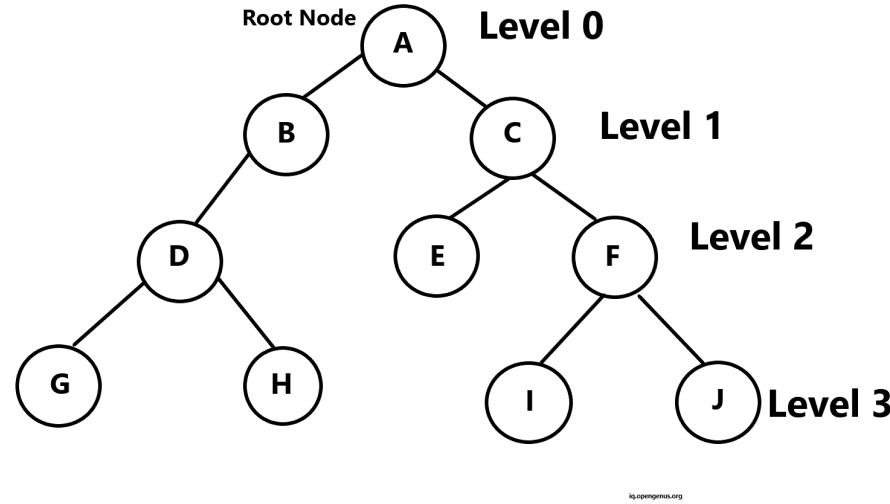
\includegraphics[width=.5\textwidth]{binary_tree}
\caption[Binary tree representation]{
  \textbf{Binary tree illustration} where the blue nodes illustrate leafs and the red node is the root of the tree.
  }
\label{fig:binary_tree}
\end{figure}

Binary trees offer several advantages over other data structures. One of the main advantages is their ability to efficiently search, insert, and delete elements. Another advantage is their simplicity and interpretability, as the structure of a binary tree is easy to understand and visualize. This makes it easier to understand how decisions are made and identify errors in the model. In the context of reinforcement learning, binary trees can provide better approximation of discontinuities by allowing for different actions depending on the chosen path. This will be one of the motivations of the project discussed later.

\section{Architecture search}

Neural networks have seen significant advancements in recent years, due in large part to the availability of vast amounts of data. Deep neural networks have demonstrated their ability to solve a wide range of problems, such as image recognition and translation. However, finding the optimal number of layers and nodes, referred to as the architecture, for a neural network to efficiently solve a problem is still a challenging task. One approach is to try different architectures and evaluate their performance, which can be time and effort consuming when dealing with deep, complex neural networks as the structure needs to be designed by hand. Another approach is to use neural architecture search (NAS), which automates the process of finding an appropriate architecture for a specific task. Researchers continue to investigate effective methods for architecture search, with evolutionary algorithms, reinforcement learning, gradient-based optimization, or a combination of these techniques, being commonly used to explore the space of possible architectures(\cite{elsken_neural_nodate}).

Until now, neural architecture search algorithms tend to be slow and expensive due to the need to train a large number of candidate networks to inform the search process. The paper by \cite{mellor_neural_nodate} showed that a possible solution to speed up this process would be to perform neural architecture search without any network training. The authors implemented a search algorithm called "NASWOT," which only makes observations on the initial untrained networks in the scope of convolutional networks.

The process of architecture search, which involves searching for structures that improve model performance without manual intervention, has been widely applied to neural networks. However, it can also be applied to binary tree models. In particular, for complex reinforcement learning tasks, a larger binary tree is usually required to increase the search space for policies and improve the probability of finding good solutions. Therefore, it is important to adapt the size of the tree according to the complexity of the task.

One approach to achieving this is by dynamically incrementing the size of the tree, using various strategies to add or remove nodes. For example, nodes could be added from left to right until the level is full and then proceed to the next layer, or they could be added to a randomly selected leaf. In this project, the latter approach is taken for this project as you will see later.

A challenge to consider is the timing at which the dynamic adaptation of the tree should occur, as changing the size of the tree too rapidly could lead to the algorithm not having enough time to search for solutions in the actual search space. Conversely, waiting too long could result in the algorithm getting stuck in a local optimum and wasting time. Therefore, it is important to strike a balance and change the size of the tree at the right moment.

Another important consideration is what functions the newly created nodes should have. Should they be the same as their parent nodes, or should they be different? This decision can have a significant impact on the performance of the model.

Finally, an unexpected consideration is whether the newly added nodes should be leaves or not. In this project, the decision is made to not add leaves, but the impact of this decision is discussed further in the project.

All of these decisions and more must be made and possibly compared when deciding which inserting strategy to implement. It is important that, even if the tree structure changes, the model remains invariant, which can be a challenging aspect to implement and can also limit the strategies that can be used.


\section{Motivation and Hypothesis for Discontinuous Models in Reinforcement Learning}

In this project, it is observed that current models are typically designed for continuous control, but many control tasks are not. Continuous control refers to tasks where the observation and action space are continuous and the control actions can take on any value within a continuous range of values. Examples of such tasks include robotic arm control and autonomous vehicle navigation. On the other hand, discontinuous control problems have discrete action spaces, which means that only a limited number of actions can be executed. Examples of such tasks include playing chess or running through a maze (\cite{sutton_reinforcement_2018}).

Neural networks, which are commonly used for modeling continuous control tasks, require continuous functions in backpropagation. The backpropagation algorithm adjusts the weights of the network by calculating the gradient of the loss function with respect to the weights. This is done by propagating the error backwards through the network, hence the name "backpropagation". The goal is to minimize the error of the network, which is repeated for many iterations until the model converges to a set of weights that minimize the error.

An example of a non-continuous control problem is the swing-up cartpole task. This task involves a pendulum fixed to a cart with a fixed joint above and a loose joint below, which is swung up in the first step and then stabilized in the second step (see Figure\ref{fig:swing_up}). When attempting to approximate the function that models this task, it becomes apparent that the function will have a discontinuity. Due to the two distinct tasks involved, the agent must be able to recognize when the first task is complete and the second one begins. In the real world, there are many control problems that are not continuous.

The hypothesis of this project is that discontinuous models would have an advantage in addressing these tasks. Binary trees are used to approximate discontinuities by using a hyperplane to partition the observation space, and depending on the chosen subtree (by going to the left or right child), a different policy will be used. To test this hypothesis, multiple individuals can be evaluated in the environment (by running them through the fitness function) and their performance analyzed, along with other metrics such as the number of individuals that successfully solve the task. Hyperparameters also play an important role in improving the performance of individuals in the environment.


\begin{figure}[!ht]
    \centering
    \begin{subfigure}{.48\textwidth}
        \centering
        \fbox{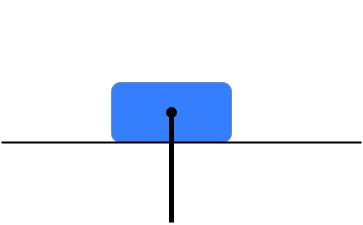
\includegraphics[width=1\linewidth]{swing_up_initial}}
        \caption{In the initial task the pole is pointing downwards and needs to be swung up by moving the blue cart on the horizontal line.} 
        \label{swing_up_initial}
    \end{subfigure}%
    \hspace{1em}
    \begin{subfigure}{.48\textwidth}
        \centering
        \fbox{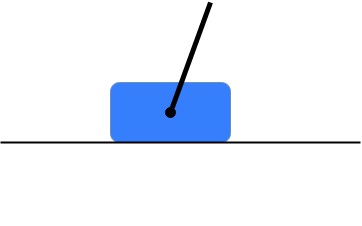
\includegraphics[width=1\linewidth]{swing_up_running}} 
        \caption{The cart has successfully managed to swing the pole up and now needs to stabilize it vertically in a second phase.} 
        \label{swing_up_running}
    \end{subfigure}
    \caption{Cart-pole swing up problem as representation of a non-continuous control task}
    \label{fig:swing_up}
\end{figure}


\section{Contribution}

This thesis builds on prior work titled "Alternative Models for Direct Policy Search in Reinforcement Learning Control Problems" (\cite{masanti_alternative_nodate}), which proposes using binary trees as an alternative to neural networks for reinforcement learning tasks. The main contributions of this work are:

\begin{itemize}
\item Refactoring the initial code provided to make it work and separating the modules into a more organized project structure.
\item Implementing CMA-ES as an optimizer for more complex problems.
\item Writing a setup to run experiments from scratch and using two environments with configuration files to make the project more customizable and easier to understand.
\item Introducing a novel function that dynamically increases the size of the binary tree, which is a crucial step towards enabling architecture search for binary trees and has the potential to significantly improve their performance in solving reinforcement learning tasks. However, only one possible tree-growing strategy will be tested, and no comparison of different structures will be made. The goal is solely to increase the tree size until the given task can be solved.
\end{itemize}

The contributions of this work aim to provide an alternative to neural networks for reinforcement learning tasks. Binary trees could potentially offer this alternative and this work aims to give a first insight into architecture search for binary trees, which could further improve their performance.